\documentclass[onecolumn,fleqn,12pt,openany]{book}
\renewcommand{\baselinestretch}{1.5}


% packages
\usepackage{ifpdf}
\usepackage{bm}
\usepackage{latexsym}
\usepackage{pstricks}
\usepackage{figsize}
\usepackage{subfigure}
\usepackage{caption}
\usepackage{hyperref}

% fonts
\usepackage{latexsym}
\usepackage{amssymb}
\usepackage{bm}
\usepackage{bbm}
%\usepackage[thinlines]{easybmat}
\usepackage{sidecap}

\usepackage{graphicx}
\usepackage{epsfig}

%%%%%%%%%%%%%%%%%%%%%%%%%%%%%%%%%%%%%%%%%%%%%%%%%%%%%%%%%%%%%%%%
%Page setup
\pagestyle{plain}
\oddsidemargin  0.0in
\evensidemargin 0.0in
\textwidth      6.5in
\headheight     0.0in
\topmargin      0.0in
\textheight     8.0in
\setlength{\parindent}{0cm}
\setlength{\parskip}{0.0cm}


%%%%%%%%%%%%%%%%%%%%%%%%%%%%%%%%%%%%%%%%%%%%%%%%%%%%%%%%%%%%%%%%
\begin{document}
\def\be{\begin{equation}}
\def\ee{\end{equation}}
\def\bea{\begin{eqnarray}}
\def\eea{\end{eqnarray}}
\def\nl{\\ \noindent}
\def\nn{\\ \nonumber}


\newcommand{\Cn}[1]{\begin{center} #1 \end{center}}

%%%%%%%%%%%%%%%%%%%%%%%%%%%%%%%%%%%%%%%%%%%%%%%%%%%%%%%%%%%%%%%%
\begin{titlepage}


\Cn{\LARGE \bf Notes on noise, diffusion and coherence\\
in biological systems\\ 
with\\
 Andrew Mugler and Tommy Byrd}



\bigskip
\bigskip


\bigskip
\bigskip
\bigskip
\bigskip
%\noindent This document ....
\bigskip
\bigskip
\Cn{
Notes by: {\bf Amir Erez}

\bigskip

}

\bigskip
\bigskip

\bigskip
\bigskip

\Cn{\today}


\end{titlepage}


\newpage

%%%%%%%%%%%%%%%%%%%%%%%%%%%%%%%%%%%%%%%%%%%%%%%%%%%%%%%%%%%%%%%%

%%%%%%%%%%%%%%%%%%%%%%%%%%%%%%%%%%%%%%%%%%%%%%%%%%%%%%%%%%%%%%%%

\newpage

{\footnotesize \tableofcontents}
\newpage

%%%%%%%%%%%%%%%%%%%%%%%%%%%%%%%%%%%%%%%%%%%%%%%%%%%%%%%%%%%%%%%%%%
%%%%%%%%%%%%%%%%%%%%%%%%%%%%%%%%%%%%%%%%%%%%%%%%%%%%%%%%%%%%%%%%%%
%%%%%%%%%%%%%%%%%%%%%%%%%%%%%%%%%%%%%%%%%%%%%%%%%%%%%%%%%%%%%%%%%%

\chapter{Questions / summary}
\section{Questions}
Below is a short summary of the questions still open in this project, ordered in order of relevance and research time-line.

\begin{enumerate}
\item Does long-range communication reduce the time needed to sense a gradient?
\item Can long-range correlation improve sensing?
\item Is/why is it useful to propagate fluctuations over large distance when sensing ?
\item How does the off-diagonal noise propagate through the nonlinear system ?
\item Can we understand disorder in terms of site or bond percolation?
\end{enumerate}

\vspace{0.5cm}

\textbf{Can feedback improve sensing precision by allowing long-range communication?}

\textit{The working hypothesis is that the most promising regime is one in which feedback gives rise to a quartic potential (to admit long-range order), but with only one basin (to eliminate sensing ambiguity).  As before, both local and global species would respond identically (but now nonlinearly) to the signal, only the global species would be exchanged, and the difference between them would be the readout.}

\vspace{0.5cm}

Below a partial list of some of the questions we've managed to answer or partially answer:

\begin{itemize}
\item Why does a nearest-neighbor Ising model allow for long-range order but nearest-neighbor diffusion doesn't ? Answer: the diffusion term simply adds a linear gradient term to the Langevin equation. The Ising systems allows fluctuations to interact with each other, which corresponds to a $y^4$ in the Landau functional or a  $y^3$ term in the corresponding Langevin equation.
\item What is the form of the correlation function we expect in an interacting/non-interacting system ? Answer: See Eq. \ref{eq:correlation_function_direct} and its solution.
\item Can feedback lead to long-range correlation? Answer: in Sec. \ref{sec:Hill_function_to_Landau} we show how a hill-function term in the LEGI equation can be recast as a $y^3$ interaction term in the Landau treatment.
\item What is the biological meaning of $\Gamma_0$ and the temperature ? How are they related ? Answer: Within the time-dependent Ginzburg-Landau theory we have $D=2\Gamma_0 k_B T$ with D the variance of the noise $\eta$ such that $P(\eta(\mathbf{r},t)) \propto \exp\left[-\frac{1}{2D}\int dt\,d^d\mathbf{r}\, \eta^2(\mathbf{r},t)\right]$. Therefore, knowing the variance of the noise gives us the value $\Gamma_0 k_B T$ in a biological setting.
\item What are the parameters of the LEGI model that go to zero at the critical point ? Partial answer: A direct treatment of the LEGI model together with the standard treatment of the Landau theory give the same correlation function. Accordingly we expect that na\"ive criticality is reached when the coefficient of the linear term in LEGI goes to zero. Taking into account Gaussian fluctuations yields corrections that suppress the critical point so that the linear term need not go to zero for criticality to set in.
\end{itemize}


\section{Summary so far}
%%%%%%%%%%%%%%%%%%%%%%%%%%%%%%%%%%%%%%%%%%%%%%%%%%%%%%%%%%%%%%%%%%%%%%%%%%%%%%%%%%%%
We have done the following:

\vspace{0.5cm}

\begin{tabular}{|c|ccc|}
\hline
Approximation & $N=1$ & $N=2$ & $N=\infty$ \\
\hline
$O(F')$ 		& Yes 	& Yes 	& Yes 	\\
$O(F'')$		& Yes 	& part 	& ? 		\\
full $F$		& Yes 	& ? 		& ? 		\\
\hline
\end{tabular}


%%%%%%%%%%%%%%%%%%%%%%%%%%%%%%%%%%%%%%%%%%%%%%%%%%%%%%%%%%%%%%%%%%%%%%%%%
\chapter{Correspondence and differences between LEGI and TDGL}
%%%%%%%%%%%%%%%%%%%%%%%%%%%%%%%%%%%%%%%%%%%%%%%%%%%%%%%%%%%%%%%%%%%%%%%%%
\label{chap:LEGI_and_Ginzburg_Landau}
In this chapter we derive the LEGI/Langevin equations from a Landau functional using the time-dependent Ginzburg-Landau (TDGL) method \cite{Hohenberg1977} ("Model A") and solve for the correlation function using a Fourier transform.

Note that:
\begin{itemize}
\item The Fourier transform method implicitly assumes spatial homogeneity. I think this comes from the employing the Weiner-Khinchine theorem but I'm not completely certain.
\item One subtlety here is the spatial-correlated nature of the noise. We briefly explore this subtlety and deduce that it should not affect the long-range behavior of the correlation function. 
\end{itemize}

\section{Species - equations of motion}
The sensing is done by two cellular molecules: local $x_n(t)$ and global $y_n(t)$ and an EGF signal $c_n$.
On the lattice they obey the following equations:
\bea 
\label{eq:LEGI_t_Langevin_eq}
c_n(t) &=& \langle c_n \rangle + \xi_c(n) \nn
\frac{d x_n}{dt} &=& \beta(c_n a^3) -\mu x_n + \xi_x(n) \nn
\frac{d y_n}{dt} &=& \beta(c_n a^3) -\mu y_n + \gamma(y_{n-1}+y_{n+1}-2y_n) + \xi_y(n) 
\eea
with noise-averaged, steady state values $\langle ... \rangle$
\bea 
\langle c_n \rangle &=& \langle c_N \rangle - ag(N-n) \nn
\langle x_n \rangle &=& G c_n a^3 \nn
G &=& \frac{\beta}{\mu}
\eea
\section{Noninteracting equation}
As we discussed, the diffusing global species obeys the following equation:

\be
\frac{\partial y(z)}{\partial t} = A_1 + A_2 y(z) + \gamma a^2 \nabla^2 y(z) + \xi_y(z)
\ee

which can be derived from an incomplete free energy functional \footnote{which is obtained by integrating over many microscopic degrees of freedom},
\be  
\mathcal{F}[y] = \int dz\, \left( \frac{a^2}{2}\left( \nabla y \right)^2 + \frac{1}{2} A_2 y^2 + A_1 y \right)
\ee
According to the TDGL/Model A rule \cite{Goldenfeld1992}\cite{Hohenberg1977},
\be
\label{eq:TDGL}
\frac{\partial y(z)}{\partial t} = -\Gamma_0 \frac{\delta \mathcal{F}}{\delta y} + \xi_y
\ee
Under the following assumptions:
\bea
\label{eq:TDGL_noise_corr}
\langle \xi_y \rangle &=& 0 \nn
\langle \xi_y(z,t) \xi_y(z',t') \rangle &=& 2\Gamma_0 \delta(x-x') \delta(t-t')
\eea

Note that the kinetic coefficient $\Gamma_0$ in the noise correlation Eq. \ref{eq:TDGL_noise_corr} is exactly the same as the one which appears in the "Model A" prescription Eq. \ref{eq:TDGL}. Taken together, the first term in Eq. \ref{eq:TDGL} causes $y$ to relax towards a configuration which minimizes the functional $\mathcal{F}(y)$ while the noise $\xi_y$ ensures that the equilibrium distribution is maintained, and that the fluctuation-dissipation theorem is satisfied \cite{Glauber1963}.

\textbf{For time-independent fields} $A_1$, there exists an equilibrium probability distribution
\bea
P_{eq}(y) &=& \frac{1}{Z} e^{-\mathcal{F}[y]} \nn
Z &=& \int \mathcal{D}y\, e^{-\mathcal{F}[y]}
\eea

\subsection{Solving the non-interacting equation in one dimension}

To solve Eq. \ref{eq:TDGL}, 
we enjoy its linearity in $y$ to introduce the Fourier transform,
\be
\label{eq:FT}
y(z,t) = \int \frac{d\omega}{2\pi}\,\frac{dk}{2\pi}\, e^{-i(kz-\omega t)} y_k(\omega)
\ee
First we tranform only the spatial part of the equation to get
\be 
\label{eq:LEGI_Langevin_eq_k_space}
\frac{\partial y_k(t)}{\partial t} = A_1 + A_2 y_k - \gamma a^2 k^2 y_k + \xi_k
\ee
which gives the steady-state value for y,
\be
\langle y_k \rangle = - \frac{\langle A_1 \rangle }{A_2 - \gamma a^2 k^2}
\ee

Next, we introduce the deviation from the steady state,
\bea
\delta y_k &=& y_k - \langle y_k \rangle \nn
\delta A_1 &=& A_1 - \langle A_1 \rangle \nn
\delta A_2 &=& A_2 \quad \mbox{(assume it doesn't fluctuate)}
\eea

Which leads to the following equation,
\be
 \frac{\partial \delta y_k(t)}{\partial t} = \delta A_1 + \left( A_2  - \gamma a^2 k^2 \right) \delta y_k + \xi_k
\ee
now we can fourier transform the time to get,
\be 
\delta y_k(\omega) = \frac{\delta A_1(\omega) + \xi_k(\omega)}{i\omega - A_2 +\gamma a^2 k^2 }
\ee
which means that, assuming $\langle \delta A_1 \xi \rangle = 0$ \footnote{The generating function dynamics (from the master equation) teach us that there is a non-zero diagonal element to this function which increases the same-species correlation. For a point source of c species at $\delta(r_1)$, the $y$ species variance has an additional term $e^{-r_2/k}$, noticed as a 'kink' at zero distance in the simulations.} , 
\be
\langle \vert y_k(\omega) \vert ^2 \rangle = \frac{\langle\vert \delta A_1(\omega) \vert ^2 \rangle}{(A_2 + \gamma a^2 k^2)^2 + \omega^2} + \frac{\langle\vert \xi_k(\omega) \vert ^2 \rangle}{(A_2 + \gamma a^2 k^2)^2  + \omega^2}
\ee
We assume that:
\bea
\langle\vert \delta A_1(\omega) \vert ^2 \rangle &=& 2\pi Q_1 \delta(\omega) \quad \mbox{ (Poisson distributed, fixed molecule number)} \nn
\langle\vert \xi_k(\omega) \vert ^2 \rangle &=& Q_2 \quad \mbox{(This needs modification in LEGI)}
\eea
which gives the time-independent, (Since $\int \frac{dw}{2\pi} \frac{1}{w^2 + a^2} = \frac{1}{2 \vert a \vert}$),
\bea
\langle \vert y_k(t) \vert ^2 \rangle &=& \int_{-\infty}^{\infty} \frac{d\omega}{2\pi} \langle \vert y_k(\omega) \vert ^2 \rangle \nn
 &=& \frac{Q_1}{(A_2 + \gamma a^2 k^2)^2 } + \frac{Q_2/2}{A_2 + \gamma a^2 k^2} 
\eea
The following integrals are useful:
\bea 
\label{eq:G_from_LEGI_1d} 
\int_{-\infty}^{\infty} \frac{dk}{2\pi} \, \frac{e^{i k x} }{b^2 + k^2} &=& \frac{1}{2\vert b \vert }e^{-\vert b x \vert } \nn
\int_{-\infty}^{\infty} \frac{dk}{2\pi}\, \frac{e^{i k x} }{(b^2 + k^2)^2} &=& e^{-\vert b x \vert } \left( \frac{\vert x \vert}{4 \vert b \vert^2} + \frac{1}{4\vert b \vert ^3 }\right)
\eea

In both cases, we see a decay in correlations with distance as $e^{-b x}$. Substituting $b^2 \propto \frac{A_2}{\gamma a^2} \propto \frac{\mu}{\gamma}$ we see that the correlations decay with a typical distance of $\sqrt{\frac{\gamma}{\mu}}$

\textbf{The apparant discrepancy:} Between Andrew's Eq. 19, where the extrinsic noise is $K_n^2$, 
\be 
\sigma_{y_N}^2 = \frac{\beta^2}{\mu^2}\sum_n{K_n^2 \bar{S}_{N-n}} + \bar{Y}_N\, ,
\ee
and the linear here, implies that the actual correlation length is $1/2$ the one derived above by,
\bea 
K_n &\approx &\frac{1}{n_o}e^{-n/n_0} \nn
\bar{S}_n &=& \alpha/\nu \, = \, \mbox{const}, \nn
\sigma_{y_N}^2 &=& \frac{\beta^2}{\mu^2}\frac{\alpha}{\nu}\sum_n{e^{-2n/n_0}}+ \bar{Y}_N\nn
	&= & \frac{\beta^2}{\mu^2}\frac{\alpha}{\nu} \frac{1}{2n_0}\sum_n{\frac{1}{n_0/2} e^{-n/n_0}} + \bar{Y}_N
\eea

\textbf{Important note:} $A_1$ is explicitly spatially dependent. By shift to the $\delta A_1$ coordinate we remove this explicit dependence but the power spectrum $\langle \vert \delta A_1 \vert ^2 \rangle$ remains spatially dependent. In such a case, it is not at all clear that we can use the Wiener-Khinchin theorem to relate the power-spectrum of the noise to the fluctuations.

\textbf{Fluctuations:} above we have calculated the distance-dependent (two-point) correlation function. To calculate fluctuations $\langle \delta y^2 \rangle$ for the one-dimensional case above, simply take the limit $x\rightarrow 0$.
\subsection{Higher dimensions}
In \textbf{two dimensions} we deal with integrals of the form,
\bea
\label{eq:G_from_LEGI_2d} 
\int_{0}^{\infty} k\, \frac{dk}{2\pi} \,  \int_{0}^{2\pi} \frac{d\phi}{2\pi}\, \frac{e^{i \vec{k}\cdot \vec{x}} }{b^2 + k^2} &=& \int_{0}^{\infty} \frac{dk}{2\pi} \frac{k J_0(kx)}{b^2 + k^2} = \frac{1}{2\pi} K_0(\vert b\vert x)\, \quad (x>0)\nn
\int \frac{d^2k}{(2\pi)^2}\, \frac{e^{i \vec{k}\cdot \vec{x}} }{(b^2 + k^2)^2} &=& \frac{x}{4\pi \vert b \vert} K_1(\vert b \vert x)\, \quad (x>0)
\eea
With $J_0$ the zeroth order Bessel $J$ function (of the first kind) and $K_0$ the modified Bessel function of the second kind. In both cases, the asymptotic expansion at $bx \gg 1$ gives \cite{AbramowitzStegun}
\be 
K_\nu(b x) \sim \sqrt{\frac{\pi}{2\vert b \vert x}} e^{-\vert b \vert x} \, , \qquad \vert b \vert x \rightarrow \infty
\ee
Again substituting $b^2 \propto \frac{A_2}{\gamma a^2} \propto \frac{\mu}{\gamma}$ we see that the correlations decay with a typical distance of $\sqrt{\frac{\gamma}{\mu}}$.

\textbf{Fluctuations:} here we must be more careful. The limit $\lim_{x\rightarrow 0} x K_1(b x) = \frac{1}{b}$ serves well to handle the second integral. However, the first integral is \emph{ultraviolet-divergent} and needs to be cut off rather than taken to infinity. This is quite easily done by noting that the "lattice constant" or "cell size" $a$ supplies a minimal wavelength $a$ and therefore a maximal wave number $k_{max} = \frac{2\pi}{a}$. Such a treatment gives the (typically logathmic) divergence of the first integral as $\ln[1 + \frac{(2\pi)^2}{a^2 b^2}]$ which indeed diverges at the (unphysical/unbiological) limit of $a\rightarrow 0$.
\vspace{1cm}

In \textbf{three dimensions} we deal with integrals of the form,
\bea
\label{eq:G_from_LEGI_3d}
\int\frac{d\vec{k}}{(2\pi)^3} \, \frac{e^{i \vec{k}\cdot \vec{x}} }{b^2 + k^2} &=& \int_{0}^{\infty} \frac{dk}{(2\pi)^2} \frac{k^2}{b^2 + k^2} \int_{-1}^{1} e^{i k r \cos\theta} d(\cos\theta) \nn
  &=& \int_{0}^{\infty} \frac{dk}{(2\pi)^2} \frac{k^2}{b^2 + k^2} \frac{2 \sin k r}{k r} \nn
  &=& \frac{1}{4\pi \vert r \vert} e^{- b r} \nn
\int \frac{d\vec{k}}{(2\pi)^3}\, \frac{e^{i \vec{k}\cdot \vec{x}} }{(b^2 + k^2)^2} &=& \frac{1}{8\pi \vert b \vert} e^{-b r}
\eea 
As before, we see the same exponential decay of correlations.

\textbf{Fluctuations:} again we must be more careful. As before, the second integral poses no problems, but the first integral diverges when $x\rightarrow 0$. Again - the UV divergence can be physically/biologically explained. This yields,
\be 
\int\frac{d\vec{k}}{(2\pi)^3} \, \frac{1 }{b^2 + k^2} = \frac{4\pi}{(2\pi)^3} \int_0^{\frac{2\pi}{a}} \frac{k^2\,dk }{b^2 + k^2} = \frac{1}{4 \pi^2}\left(1/a - b \cot^{-1} ab \right)
\ee
The above integral diverges more dramatically as $\frac{1}{a}$ when the lattice/cell size $a$ is artificially taken to zero.

\section{Discrete case}
What happens when instead of the continuum limit taken above, we use the lattice description (which is more suitable to cells). Below we will see that the only difference is that in Fourier space instead of $k^2$ we have $\cos(ka)$.

\subsection{A note about periodic boundary conditions}
For mathematical convenience we use periodic boundary conditions. To accommodate the spatial gradient in the EGF we change to the geometry described in Fig. \ref{fig:Periodic_1d_lattice}.

\begin{figure}[!ht]
 \centering
  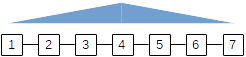
\includegraphics[clip,width=0.49\hsize]{Periodic_1d_lattice.png}
  \caption{Periodic 1-d lattice with EGF gradient. For the non-periodic lattice: $N=4$. Here, we extend the lattice up to $2N-1=7$ sites with $c_{2N-1}=c_1$.}
  \label{fig:Periodic_1d_lattice}
\end{figure}

Using the spatial dependence of the EGF signal,
\be 
c_n = \left\{ \begin{array}{ll}
		c_N-ag(N-n) & 1\le n \le N \\
		c_N-ag(n-N) & N\le n\le 2N-1 \\
\end{array} \right.
\ee
\subsection{Gillespie derivation of the noise power-spectrum}
A simple way to derive the off-diagonal noise is by using Gillespie's formalism \cite{Gillespie2000}. 
We define the \emph{species} $y_1,y_2,...$ as the $y$ molecule concentrations in the different lattice sites. We also define the \emph{reactions} $r_k$ as all the possible fluxes/rates (in units of time$^{-1}$) such that,
\be
\frac{\partial y_j}{\partial t} = \sum_m A_{jm} r_m + \sum_m A_{jm}\sqrt{\langle r_m \rangle} \eta_m
\ee
Where we have assumed the noise in reaction space $\eta_m$ is approximately Gaussian with a Poisson $\sqrt{\mbox{mean}}$ standard deviation and diagonal such that,
\bea
\langle \eta_m \rangle &=& 0 \nn
\langle \eta_m(t) \eta_n(t') \rangle &=& \delta(t-t')\delta_{m,n}
\eea

\vspace{0.5cm}

Assuming periodic boundary conditions, we can define the stoichiometric matrix $A_{jk}$,
(for a 4-species example below),
\be 
A_{jk} = \left( \begin{array}{cccc|cccc|cccc|cccc} 
	+1 & -1 & +1 & -1 & -1 & +1 &  0 &  0 &  0 &  0 &  0 &  0 &  0 &  0 &  0 &  0 \\
	0  &  0 &  0 &  0 & +1 & -1 & +1 & -1 & -1 & +1 &  0 &  0 &  0 &  0 &  0 &  0 \\
	0  &  0 &  0 &  0 &  0 &  0 &  0 &  0 & +1 & -1 & +1 & -1 & -1 & +1 &  0 &  0 \\
	-1 & +1 &  0 &  0 &  0 &  0 &  0 &  0 &  0 &  0 &  0 &  0 & +1 & -1 & +1 & -1 \\	
\end{array} \right)
\ee
with the reactions ordered as follows: 

$y_4\rightarrow y_1 ; y_1\rightarrow y_4 ; \varnothing \rightarrow y_1 ; y_1\rightarrow \varnothing$

$y_1\rightarrow y_2 ; y_2 \rightarrow y_1 ; \varnothing \rightarrow y_2 ; y_2 \rightarrow \varnothing $

$...$ 

So that the rates are,
\be 
\vec{r} = \left( \begin{array}{c}
	\gamma y_4 \\
	\gamma y_1 \\
	\beta c_1 a^3 \\
	\mu y_1 \\
	\hline \gamma y_1 \\
	\gamma y_2 \\
	\beta c_2 a^3 \\
	\mu y_2 \\
	\hline \gamma y_2 \\
	\gamma y_3 \\
	\beta c_3 a^3 \\
	\mu y_3 \\
	\hline ... \\
\end{array} \right)
\ee

So that, focusing on $y_2$, we have,
\bea
\frac{\partial y_2}{\partial t} &=& \left( \beta c_2 a^3 - \mu y_2 - 2 \gamma y_2 + \gamma y_1 + \gamma y_3  \right) \nn
 &+& \left( \sqrt{\beta \langle c_2 \rangle a^3}\eta_5 - \sqrt{\mu \langle y_2 \rangle}\eta_6 - \sqrt{\gamma \langle y_2\rangle }\eta_2 + \sqrt{\gamma \langle y_1\rangle }\eta_3 - \sqrt{\gamma \langle y_2\rangle }\eta_7 + \sqrt{\gamma \langle y_3\rangle }\eta_8\right) \nn
 &=& \left( \beta c_2 a^3 - \mu y_2 - 2 \gamma y_2 + \gamma y_1 + \gamma y_3  \right) + \xi_y(2,t)
\eea
Where the first term in the parenthesis is the deterministic evolution and the second term is the stochastic noise. We immediately see that the stochastic noise in \emph{species} space now has off-diagonal correlations,
\be 
\langle \xi_y(2,t) \xi_y(2,t) \rangle = \left( \beta \langle c_2  \rangle a^3 + \mu \langle y_2 \rangle + 2 \gamma \langle y_2 \rangle  + \gamma \langle y_1 \rangle + \gamma \langle y_3 \rangle  \right)
\ee

\subsection{Alternative derivation for linear reactions}
In a purely model which is linear in the species $y_n$, we can use a more direct formalism 

\bea
\label{eq:discrete_pbc_evolution}
\frac{\partial y_j}{\partial t} &=& \left[ (-2\gamma -\mu) \hat{I}_4 + \gamma\,\left( \begin{array}{cccc}
0 & 1 & 0 & 1 \\
1 & 0 & 1 & 0 \\
0 & 1 & 0 & 1 \\
1 & 0 & 1 & 0 \\ 
\end{array} \right) \right]
\left( \begin{array}{c}
	y_1 \\
	y_2 \\
	y_3 \\
	y_4 \\
\end{array} \right) +\beta a^3 \left( \begin{array}{c}c_1 \\ c_2 \\ c_3 \\ c_4 \end{array} \right) \nn
 &+& \mbox{noise}
\eea

We define the translation operator $\hat{D}$ such that when it works on the localized state $\vert n \rangle$,
\bea 
\hat{D} \vert n \rangle &=& \vert n +1 \rangle \nn
\hat{D}^{\dag} \vert n \rangle &=& \vert n-1 \rangle
\eea

We can define the momentum states $\vert k_n \rangle$ with $k_n = \frac{2\pi a n}{2N-1}$ such that,
\bea 
\label{eq:k_basis}
\vert k_n \rangle  &=& \frac{1}{\sqrt{2N-1}}\sum_m e^{i k_n m} \vert m \rangle \nn
\vert n \rangle  &=& \frac{1}{\sqrt{2N-1}}\sum_k e^{-i k n} \vert k \rangle
\eea
Where these momentum states are eigenstates of the translation operator,
\bea 
\hat{D}\vert k_n \rangle &=& e^{i k_n} \vert k_n \rangle \nn
\hat{D}^\dag \vert k_n \rangle &=& e^{-i k_n} \vert k_n \rangle
\eea
Defining the vectors $\vert y \rangle = \sum_{n=1}^{2N-1}y_n\vert n \rangle$ and $\vert c \rangle = \sum_{n=1}^{2N-1}c_n\vert n \rangle$, etc., the equation of motion Eq. \ref{eq:discrete_pbc_evolution} can be written as,
\bea 
\frac{\partial}{\partial t} \vert y \rangle &=& \left[ \left( -2\gamma -\mu\right) \hat{I}_{2N-1} +\gamma \left(\hat{D}+\hat{D}^\dag \right)\right] \vert y \rangle +\beta a^3 \vert c \rangle + \vert \xi_y \rangle
\eea
Substituting the relation Eq. \ref{eq:k_basis}, we get,
\bea 
\forall &k: & \sum_{n=1}^{2N-1} e^{i k n} \left[\left(\frac{\partial}{\partial t} + 2\gamma + \mu - 2\gamma\cos{k} \right)y_n  - \beta a^3 c_n -\xi_n \right] = 0 \nn
 &\rightarrow & \left(\frac{\partial}{\partial t} + 2\gamma + \mu - 2\gamma\cos{k} \right)\tilde{y}_k  - \beta a^3 \tilde{c}_k -\tilde{\xi}_k = 0
\eea
This is the discrete from of the Fourier tranform \ref{eq:LEGI_Langevin_eq_k_space} of Langevin Eq. \ref{eq:LEGI_t_Langevin_eq}.

%%%%%%%%%%%%%%%%%%%%%%%%%%%%%%%%%%%%%%%%%%%%%%%%%%%%%%%%%%%%%%%%%%%%%%%%%5
\section{Correlated Noise}
The noise power-spectrum in the LEGI model shows off-diagonal terms. In this section we derive these terms and then explore how the off-diagonal elements modify the results of the previous section.


\subsection{Back to LEGI}
Let us go back to the k-space expression for the noise fluctuations from the previous section,
\be 
\langle\vert \xi_k(\omega) \vert ^2 \rangle = Q_2 \quad \mbox{(This needs modification in LEGI)}
\ee
Indeed - as mentioned, this term needs modification. Going back to the Gillespie method \cite{Gillespie2000} we see that for the diffusing species, the noise-noise correlation follows:
\bea
\langle \xi_n(t)\xi_m(t')\rangle &=& \delta(t-t')\left[ \left( A_1 + A_2 + B_-+B_+\right) \delta_{n,m} - B_-\delta_{m,n-1} - B_+\delta_{m,n+1} \right] \nn
B_- &=& B_-(n) = \gamma \langle y_n+y_{n-1} \rangle \nn
B_+ &=& B_+(n) = \gamma \langle y_n+y_{n+1} \rangle
\eea
With $\delta_{n,m}$ the Kronecker delta and $A_1(n) = \beta \langle \delta c_n \rangle a^3$ and $A_2(n) = \mu \langle \delta y_n \rangle$ are both explicitly dependent on the location index $n$ as before. 
\vspace{1cm}

The presence of the off-diagonal terms $\delta_{m,n\pm 1}$ is unusual and is a result of the stoichiometric matrix and the assumption that the noise is diagonal-correlated in "reaction space" rather than in "real-space".

Let us define the Fourier series,
\be 
\xi_k = \frac{1}{\sqrt{N}}\sum_n e^{i k n}\, \xi_n
\ee

which means the correlation function is,
\bea
\langle \vert \xi_k \vert ^2 \rangle &=& \langle \xi_k \xi_{-k} \rangle = \frac{1}{N} \sum_{n,m} e^{ik(n-m)}\langle \xi_n \xi_m^* \rangle \nn
&=& \frac{1}{N} \sum_{n,m} e^{ik(n-m)} \left[ (A_1+A_2 + B_- + B_+ )\delta_{n,m} - B_- \delta_{m,n-1} - B+\delta_{m,n+1} \right]\nn
\eea
\vspace{0.5cm}
At this point we may introduce \emph{periodic boundary conditions} which will render the above sums easier to handle. Physically this means nothing since we've been probing a regime where correlations decay exponentially with distance, meaning that for a long enough loop, the periodicity will affect nothing. Using the periodicity, we note that the spacial average,
\be 
\frac{1}{N} \sum_n B_- = \frac{1}{N} \sum_n B_+ = \bar{B} = \frac{2\gamma}{N} \sum_n \langle y_n \rangle
\ee

\vspace{0.5cm}
Finally, we see that the diagonal terms become spatial averages,
\be
\frac{1}{N} \sum_{n,m} e^{ik(n-m)} (A_1+A_2 + B_- + B_+ )\delta_{n,m} = \frac{1}{N} \sum_{n} (A_1+A_2 + B_- + B_+ )
\ee
whereas the off-diagonal terms receive a cosine,
\bea 
\frac{1}{N} \sum_{n,m} e^{ik(n-m)}B_-(n) \delta_{m,n-1} &=& \frac{\gamma}{N} \sum_{n} e^{ik}(\langle y_n \rangle +\langle y_{n-1}\rangle) \nn
  &=& e^{ik} \frac{1}{N} \sum_n  B_- \nn
\frac{1}{N} \sum_{n,m} e^{ik(n-m)}B_+(n) \delta_{m,n+1}  &=& e^{-ik} \frac{1}{N} \sum_n  B_+ \nn
\mbox{both terms} & \rightarrow & \frac{4\gamma \cos k}{N} \sum_n \langle y_n \rangle
\eea
So that we can find the k-space noise-noise correlation,
\bea
\langle \vert \xi_k \vert ^2 \rangle &=& \frac{1}{N}\sum_n\left[A_1 + A_2 + 4\gamma(1-\cos k)\langle y_n \rangle \right] \nn
&=& Q_2 + Q_3 \cos ka 
\eea
\vspace{1cm}

\textbf{Crucially, comparing with the original hypothesized diagonal noise},  
\be 
\langle\vert \xi_k(\omega) \vert ^2 \rangle = Q_2 \quad \mbox{(non-LEGI)}
\ee
\textbf{we note the addition of an explicitly $\cos k$-dependent term}. How will this term affect the correlation functions derived above ? The effect is only on one of the integrals, transforming it so that,
\bea 
\int_{-\infty}^{\infty} \frac{dk}{2\pi} \, \frac{e^{i k x} }{b^2 + k^2} &\longrightarrow &  \int_{-\infty}^{\infty} \frac{dk}{2\pi} \, \frac{e^{i k x}\cos ka }{b^2 + k^2} \nn
 & \longrightarrow & \frac{1}{2} \int_{-\infty}^{\infty} \frac{dk}{2\pi} \, \frac{e^{i k x} (e^{ika} + e^{-ika})}{b^2 + k^2} \nn
 & \longrightarrow & \frac{1}{2} \int_{-\infty}^{\infty} \frac{dk}{2\pi} \, \frac{(e^{ik(x-a)} + e^{-ik(x+a)})}{b^2 + k^2} \nn
\eea
\textbf{Therefore the cosine term merely shifts the correlation function by a unit distance $a$, otherwise not modifying its behavior.}


\section{Introducing non-linearity}
\label{sec:Hill_function_to_Landau}
We introduce non-linearity using a hill function of order $n$,
\be 
\dot{y} = a-\mu y + \beta \frac{y^n}{y^n+k^n} + \xi_y
\ee
Expanding about $y=y^*(1+\phi)$ which is a steady-state solution to the equation,
\bea
\dot{\phi} &=& h - r\phi - v\phi^2 - u\phi^3 \nn
h &=& \frac{\alpha}{k} + \frac{\beta}{2k} - \mu \nn
r &=& \mu - \frac{n\beta}{4k} \nn
v &=& \frac{n \beta}{8k} \nn
u &=& \left(\frac{n^2}{4}-1 \right)\frac{n\beta}{12k}
\eea
If $h=0$ then $y^*=k$  \\
If $\frac{\delta F}{\delta \phi} = \langle \dot{y} \rangle = 0$ and $h=0$ then we can solve $\phi(r+v\phi+u\phi^2)=0$.
%%%%%%%%%%%%%%%%%%%%%%%%%%%%%%%%%%%%%%%%%%%%%%%%%%%%%%%%%%%%%%%%%%%%%%%%%%%%


%%%%%%%%%%%%%%%%%%%%%%%%%%%%%%%%%%%%%%%%%%%%%%%%%%%%%%%%%%%%%%%%%%%%%%%%%%%%%%%%%%%%%%%%%
\chapter{Critical phenomena in Landau theory - simple}
%%%%%%%%%%%%%%%%%%%%%%%%%%%%%%%%%%%%%%%%%%%%%%%%%%%%%%%%%%%%%%%%%%%%%%%%%%%%%%%%%%%%%%%%%
\label{chap:Critical_Landau}
We begin this chapter with a quick recap of critical behavior of Ising systems. Such critical behavior has been linked to various biological systems \cite{Krotov2014}. In the second part of this chapter we present an alternative derivation of the two-point correlation function as a function of distance, and solve it in direct rather than Fourier space. The resulting correlation function, $G(r)$, matches the ones derived in Chap. \ref{chap:LEGI_and_Ginzburg_Landau}.

\section{Correlation function and length}
We define the reduced temperature which vanishes in the thermodynamic limit,
\be
t = \frac{T-T_c}{T_c}
\ee
It can be shown that the following thermodynamic observables behave as power-laws near the phase transition,

\begin{tabular}{|l|l|l|l|l|}
\hline
Name						& Observable & 2D Ising & 3D Ising & Measurement \\
\hline
heat capacity			& $c_v \sim \vert t \vert^{-\alpha}$ & $\alpha = 0$ & 0.11&$c_v = \frac{N}{k_bT^2}\left(\langle E^2\rangle - \langle E \rangle^2 \right)$ \\
magnetization			& $m \sim \left\{ \begin{array}{ll}
							(-t)^{\beta} & T<T_c \\
							0			 & T>T_c \\
						   \end{array}\right. $ & $\beta = 1/8 $  & 0.325 & $m = \frac{1}{N}\sum_i S_i $\\
magnetic susceptibility	& $\chi \sim \vert t\vert ^{-\gamma}$ & $\gamma = 7/4$ & 1.24 &$\chi = \frac{N}{k_B T}\left(\langle M^2\rangle - \langle M \rangle^2 \right)$\\
magnetization			& $M(T_c,H) \sim H^{1/\delta}$ & $\delta = 15$ & 4.82 &at $T_c = 2.269$\\
correlation length 		& $\xi \sim \vert t \vert ^{-\nu}$ & $\nu = 1$ & 0.63 &from $g(r)$\\
pair correlation			& $g(r) \sim \frac{1}{r^{d-2+\eta}}\,e^{-r/\xi}$ & $\eta = 1/4$ & 0.032 &  $g(r) = \langle S_i S_{i+r} \rangle - \langle S_i \rangle \langle S_{i+r} \rangle $\\
\hline
\end{tabular}

\vspace{1cm}
Here is a comparison between the "real" Ising model exponents and their mean-field values,
\be 
\begin{array}{|l|l|l|l|}
\hline
\mbox{Exponent} & \mbox{True 2D value} & \mbox{True 3D value} & \mbox{MF value} \\
\hline
\alpha	& \log	& 0.11 & 0 \\
\beta	& 1/8	& 0.325 & 1/2\\
\gamma	& 7/4 	& 1.24 & 1\\
\delta	& 15		& 4.82 & 3 \\
\nu	& 1 & 0.63 & 1/2 \\
\eta		& 1/4	& 0.032 & 0 \\
\hline
\end{array}
\ee


\vspace{1cm}


\textbf{Divergence of the Susceptibility:} the susceptibility per spin when $T>T_c$ and $H=0$ is,
\bea
k_B T \chi &=& \frac{1}{N}\left( \langle M^2 \rangle - \langle M \rangle^2 \right) \nn
          &=& \frac{1}{N} \sum_{i,n} \langle S_i S_n \rangle \nn
          &\sim & \int dr\,r^{d-1} g(r) \nn
          &\sim & \int dr\,r^{d-1} r^{2-d-\eta} e^{-r/\xi} \nn
          &\sim & \int_0^{\xi} dr\, r^{1-\eta} \sim \xi^{2-\eta} \sim t^{-\nu(2-\eta)} \sim t^{-\gamma}
\eea
where we have relied on translational invariance to simplify the expression $\langle S_i S_n \rangle$. This gives us one of the scaling relations, $ \gamma = \nu(2-\eta)$.

\vspace{1cm}

\textbf{Finite size scaling:} the basic argument for finite size scaling is that near $T_c$ the correlation length $\xi$ approaches the linear size L of the system. In this
scaling region dimensionless physical quantities depend not on $\xi$ and $L$
separately but only on the ratio $L/\xi$. Accordingly, the dimensionless ratio,
\bea
\frac{\chi(T,L)}{\chi(T,\infty)} &=&  f(L/\xi) \\
\chi(T, L) &\sim & t^{-\gamma} f (L t^\nu ) = L^{\gamma/\nu} (L^{1/\nu} t)^{- \gamma} f (Lt^\nu ) \nn
&\sim & L^{\gamma/\nu}\phi(L^{1/\nu} t)
\eea

\section{Correlation function - Landau mean field}
Here we calculate the 2-point correlation function directly from Landau functional (See Chap. 5.7 in Goldenfeld \cite{Goldenfeld1992}). Our starting point is the Landau functional, 
\be 
L[y(\mathbf{r})] = \int d^d\mathbf{r} \, \left[\frac{\gamma}{2}\left(\nabla y \right)^2 + \frac{1}{2}a_2y^2 + \frac{1}{4}a_4y^4 - H(\mathbf{r})y(\mathbf{r}) \right]
\ee
which is not the Helmoltz free energy, but has mathematically similar properties to it, and can be called an 'incomplete free energy'.
 
We define the partition function,
\be 
Z = \int \mathcal{D}y\, e^{-\beta L[y(\mathbf{r})]} = e^{-\beta F}
\ee
For the sake of clarity we explicitly define the functional derivative, 
\be 
\frac{\delta F}{\delta y(\mathbf{r}')} = \lim_{\epsilon\rightarrow 0}{\frac{F[y(\mathbf{r})+\epsilon\delta(\mathbf{r}-\mathbf{r}')] - F[y(\mathbf{r})]}{\epsilon}}
\ee
Since $F = -\frac{1}{\beta}\ln Z$ we have,
\bea
\langle y(\mathbf{r}) \rangle &=&  -\frac{\delta F}{\delta H(\mathbf{r})} \nn
\chi_T(\mathbf{r},\mathbf{r}') &=& -\frac{\delta^2 F}{\delta H(\mathbf{r})\delta H(\mathbf{r}')} \nn
    &=& \frac{1}{\beta}\left( \frac{1}{Z} \frac{\delta^2 Z}{\delta H(\mathbf{r})\delta H(\mathbf{r}')} - \frac{1}{Z} \frac{\delta Z}{\delta H(\mathbf{r})}\frac{1}{Z} \frac{\delta Z}{\delta H(\mathbf{r}')}  \right) \nn
    &=& \frac{1}{\beta}\left(\langle y(\mathbf{r})y(\mathbf{r}')\rangle - \langle y(\mathbf{r})\rangle \langle y(\mathbf{r}')\rangle  \right) \nn
    &=& \beta G(\mathbf{r},\mathbf{r})
\eea
We will take the functional derivative in two steps, first we find $y_0(\mathbf{r})$ which extremizes the Landau functional,
\be 
\label{eq:y_0_from_extremum}
\left. \frac{\delta L}{\delta y(\mathbf{r})}\right\vert_{y(\mathbf{r})=y_0(\mathbf{r})} = 0 = -\gamma \nabla^2 y_0(\mathbf{r}) + a_2 y_0(\mathbf{r}) + a_4 y_0^3(\mathbf{r}) - H(\mathbf{r})
\ee
Next we perform the second derivative with respect to the source field $H(\mathbf{r}')$,
\be
\frac{\delta }{\delta H(\mathbf{r}')}\left( -\gamma \nabla^2 y_0(\mathbf{r}) + a_2 y_0(\mathbf{r}) + a_4 y_0^3(\mathbf{r}) - H(\mathbf{r}) \right)  = 0
\ee
Since $\frac{\delta H(\mathbf{r})}{\delta H(\mathbf{r}')}=\delta(\mathbf{r}-\mathbf{r}')$, we have,
\be 
\label{eq:G_with_y0}
\left(-\gamma \nabla^2 + a_2 + 3a_4 y_0^2 \right)G(\mathbf{r},\mathbf{r}') = \delta(\mathbf{r}-\mathbf{r}')
\ee
Indeed we see that the 2-point correlation function is a Green's function. We proceed to solve the equation above to derive the explicit form of the correlation function.

\subsection{Mean-field theory vs. Gaussian theory}
A subtle point here is the difference between the mean-field approach and a Gaussian approach. Explicitly, the mean field approach assumes that,
\be 
y(\mathbf{r}) = y_0(\mathbf{t})
\ee
with $y_0$ the value of the "order parameter" that extremizes the Landau functional $L$. For a uniform system at $T>T_c$ this corresponds to $y_0 = 0$ whereas for $T<T_c$ it's $y_0 = \sqrt{-a_2/a_4}$. 

\vspace{0.25cm} 

In contrast, the Gaussian theory expands the functional $L[y(\mathbf{r})]$ about its minimum,

$y(\mathbf{r}) = y_0(\mathbf{r}) + \delta y$ 

to quadratic order, neglecting the quartic term altogether, ie., setting $a_4=0$. This can work for $T>T_c$ but cannot be extended to $T<T_c$ because in that regime the quartic term is necessary to stop the functional $L$ from diverging at large $y$.

\subsection{Translationally invariant system}
In a translationally invariant system we can replace $y_0^2$ by its value from Landau theory. Therefore for $T>T_c$ we have $\langle y \rangle = 0$ and 
\bea
\left( -\nabla^2 + \xi_>^{-2}\right)G(\mathbf{r}-\mathbf{r}') &=& \frac{1}{\beta \gamma} \delta(\mathbf{r}-\mathbf{r}') \nn
\xi_>^{-2} &=&  \frac{a_2}{\gamma} \quad \,\,\,\quad(T>T_c )
\eea
For $T<T_c$ we have $\langle y \rangle = \pm \sqrt{\frac{-a_2}{a_4}}$ so that,
\bea
\left( -\nabla^2 + \xi_<^{-2}\right)G(\mathbf{r}-\mathbf{r}') &=& \frac{1}{\beta \gamma} \delta(\mathbf{r}-\mathbf{r}') \nn
\xi_<^{-2} &=&  \frac{-2 a_2}{\gamma} \quad \,\,\,\quad(T<T_c)
\eea
In both cases, since $a_2 \propto \frac{T-T_c}{T_c}$ we have the divergence of the correlation length with temperature as the usual $\nu=1/2$ mean-field value ,
\be 
\xi \sim \left(\frac{T-T_c}{T_c} \right)^{-1/2} \sim \left(\frac{T-T_c}{T_c} \right)^{-\nu}
\ee
The above Green's function can be solved in Fourier space quite easily.
Without resorting to Fourier transform (to maintain generality of solution method), we can switch to polar coordinates,
\be
\left[ -\frac{1}{r^{d-1}}\frac{\partial}{\partial r} r^{d-1}  \frac{\partial}{\partial r} + \xi^{-2}\right]G(r) = \frac{1}{\beta \gamma}\delta(r)
\ee
We scale all distances in units of the correlation length, $\rho = r/\xi$ so that $G(r/\xi) = \mathcal{G}(\rho)$, and noting that $\delta(\rho \xi)= \frac{1}{\xi^d}\delta(\rho)$ we get,
\bea
\label{eq:correlation_function_direct}
\left[-\frac{1}{\rho^{d-1}}\frac{\partial}{\partial \rho}\rho^{d-1} \frac{\partial}{\partial \rho} +1\right]\mathcal{G}(\rho)  &=& g\delta(\rho) \nn
g &=& \frac{1}{\beta \gamma}\xi^{2-d}
\eea
We note that Eq. \ref{eq:correlation_function_direct} is the spherical Bessel equation which is solved to give modified spherical Bessel functions of the third kind \cite{AbramowitzStegun} $K_n(\rho)$, 
\be 
\frac{1}{g}\mathcal{G}(\rho) = \left\{ \begin{array}{ll}
 e^{-\rho} & d=1 \\
 \frac{1}{(2\pi)^{d/2}}\frac{1}{\rho^{d/2-1}}K_{d/2-1}(\rho) & d\ge 2 \\
\end{array}\right.
\ee
Substituting for $g(\rho)$ from Eq. \ref{eq:correlation_function_direct}, we get,
\be 
\mathcal{G}(\rho) = \frac{k_B T}{\gamma} \left\{ \begin{array}{ll}
\frac{1}{r^{d-2}} \left[ \rho^{d-2} e^{-\rho} \right]& d=1 \\
 \frac{1}{r^{d-2}} \left[\frac{1}{(2\pi)^{d/2}} \rho^{(d-2)/2} K_{(d-2)/2}(\rho) \right]& d\ge 2 \\
\end{array}\right.
\ee

Using the expansions,
\be 
\begin{array}{lclcl}
\rho^{(d-2)/2} K_{(d-2)/2}(\rho) & \sim & \sqrt{\frac{\pi}{2}} \rho^{(d-3)/2} e^{-\rho}\left(1+O(1/\rho)\right), & \rho\rightarrow \infty & T\ne T_c \\
          & \sim & \frac{\Gamma((d-2)/2)}{2^{2-d/2}}\left(1+O(\rho^{d-2})\right), & d>2;\rho\rightarrow 0 & T \rightarrow T_c \\
K_0(\rho)  & \sim & \tilde{\gamma}-\ln\frac{\rho}{2}, & d=2;\rho\rightarrow 0 & T \rightarrow T_c \\          
\end{array}
\ee
with $\tilde{\gamma}$ the Euler-Mascheroni constant and $\Gamma(n)\sim (n-1)!$ the usual gamma function.

Collecting everything we have,
\bea 
G(r/\xi \gg 1;T\ne T_c) &\sim & \left(\frac{k_B T}{\gamma}\right) \frac{e^{-r/\xi}}{r^{d-2}}\left\{ \begin{array}{ll}
\frac{1}{r/\xi} & d=1 \\
\frac{1}{\sqrt{8\pi}}\frac{1}{\sqrt{r/\xi}} & d=2 \\
\frac{1}{4\pi} & d=3 \\
\end{array}\right. \nn
G(r/\xi \ll 1;T\rightarrow T_c) &\sim & \left(\frac{k_B T}{\gamma}\right)\frac{1}{r^{d-2}}\left\{ \begin{array}{ll}
\frac{1}{r/\xi}\,e^{-r/\xi} & d=1 \\
\frac{1}{2\pi}\left(\tilde{\gamma}-\ln\frac{r/\xi}{2} \right) & d=2 \\
\frac{1}{4\pi} & d=3 \\
\end{array}\right. \nn
\eea

\textbf{Comparison with Langevin approach:}

Let us compare our results from the direct approach to the derivation from the LEGI/Langevin treatment of Chap. \ref{chap:LEGI_and_Ginzburg_Landau}. The LEGI treatment was away from criticality so we are interested in comparing the $r/\xi \gg 1$ limit which is the long-distance behavior of the correlation function. Moreover, in the simplistic treatment above we didn't include the "source" species which means that in comparison with the LEGI derivation we must take $Q_1=0$ and compare only the $Q_2$ integrals. Doing that, and substituting for the correct values of the dimension $d$, we see that the two calculations (thankfully) agree.

\vspace{0.5cm}

\begin{tabular}{|c|c|c|c|}
\hline
Dim & Landau 			& LEGI 				& Where \\
\hline
1  	& $\xi e^{-r/\xi}$		& $\xi e^{-r/\xi}$		& Eq. \ref{eq:G_from_LEGI_1d} \\
2  	& $K_0(r/\xi)$			& $K_0(r/\xi)$	     	& Eq. \ref{eq:G_from_LEGI_2d} \\
3 & $\frac{1}{r}e^{-r/\xi}$ &	$\frac{1}{r}e^{-r/\xi}$	& Eq. \ref{eq:G_from_LEGI_3d} \\		
\hline
\end{tabular} 


\vspace{0.5cm}
\textbf{Notes:}
\begin{itemize}
\item The form $G(r) \sim \frac{1}{r^{d-2+\eta}}\,e^{-r/\xi}$ is preserved with $\eta=0$ . The anomalous exponent $\eta$ is zero in such a mean-field treatment. Renormalization group flow to the "Wilson-Fisher" fixed point is the only method I am currently aware of to approximate the experimentally observed values of $\eta$. Interestingly, the fact that $\eta\ne 0$ stems from the existance of a microscopic length-scale in the physics. Although the microscopic details do not matter, the existence of another length-scale is crucial to create a finite $\eta$.
\item Adding Gaussian fluctuations, ie. taking $y = y_0(\mathbf{r})+\delta y(\mathbf{r})$ and calculating $\langle y^2 \rangle$ in the path integral but truncating the treatment of the $y^4$ term, does not change the values of the critical exponents or scaling functions we have calculated. Indeed, the only difference is a correction to the specific heat exponent $\alpha$ from zero to $2-d/2$. At $d=4$, $\alpha=0$ and the Gaussian theory predicts the mean-field exponent.
\item The Bessel equation can be solved directly using Frobenius series, but a Fourier transform in suitable systems will converge to the same solution. 
\item In the presence of a "source/magnetic field" term the correlation function takes the form, (with $t=\frac{T-T_c}{T_c}$),

\be 
G(r,t,h) = \frac{1}{r^{d-2+\eta}} F \left( rt^\nu,h/t^{\beta+\gamma} \right) = \frac{1}{r^{d-2+\eta}} F \left( \frac{r}{\xi},h\xi^{(\beta+\gamma)/\nu} \right)
\ee
In our case, we can take $t\propto \mu$ the coefficient of the linear term in the Langevin equation.
\end{itemize}

\subsection{Inhomogeneous system}
Going back to Eq. \ref{eq:G_with_y0},
\be
\left(-\gamma \nabla^2 + a_2 + 3a_4 y_0^2 \right)G(\mathbf{r},\mathbf{r}') = \delta(\mathbf{r}-\mathbf{r}')
\ee
We now cannot benefit from substituting $y_0^2$ by its homogeneous Landau theory value. Instead, we must first solve Eq. \ref{eq:y_0_from_extremum},
\be 
\left. \frac{\delta L}{\delta y(\mathbf{r})}\right\vert_{y(\mathbf{r})=y_0(\mathbf{r})} = 0 = -\gamma \nabla^2 y_0(\mathbf{r}) + a_2 y_0(\mathbf{r}) + a_4 y_0^3(\mathbf{r}) - H(\mathbf{r})
\ee
Again, assuming radial symmetry we can reduce the equation to its radial components,
\be 
\left[-\frac{1}{r^{d-1}}\frac{\partial}{\partial r}r^{d-1}\frac{\partial}{\partial r} +a_2 \right]y_0 + a_4 y_0^3 = H(r)
\ee
The above equation does not seem to have a general solution. So instead, we can try a Gaussian treatment.

... To be continued.
%%%%%%%%%%%%%%%%%%%%%%%%%%%%%%%%%%%%%%%%%%%%%%%%%%%%%%%%%%%%%%%%%%%%%%%%%%%%


%%%%%%%%%%%%%%%%%%%%%%%%%%%%%%%%%%%%%%%%%%%%%%%%%%%%%%%%%%%%%%%%%%%%%%%%%%%%%%%%%%%%%%%%%
\chapter{Correlation function in homogeneous Langevin system with two noise terms}
%%%%%%%%%%%%%%%%%%%%%%%%%%%%%%%%%%%%%%%%%%%%%%%%%%%%%%%%%%%%%%%%%%%%%%%%%%%%%%%%%%%%%%%%%
\label{chap:Correlations_Langevin}
In this chapter we derive the Langevin dynamics from a Time-dependent-Ginzburg-Landau (TDGL) prescription. Such formalism requires that the noise terms are introduced by hand. We create a hybrid model A/B noise with two noise terms: one "thermal" and one "diffusional". We proceed to derive the equal-time correlation function with corrections due to diffusion. 

\section{Lagrangian and equation of motion in one dimension}
\subsection{Lagrangian}
We define the usual Ginzburg-Landau Lagrangian, to quadratic order in the zero-mean molecule density $\delta y$,
\be 
\label{eq:Lagrangian_gauss}
L = \int dx\, \left[\left(\nabla \delta y\right)^2 +\frac{a_2}{2}(\delta y)^2 + O(\delta y ^4)\right]
\ee
with the definitions,
\bea 
\langle ... \rangle &=& \mbox{Average over noise realizations} \nn
\langle y \rangle_{\mbox{noise}} &=& \bar{y} \nn
\delta y &=& y - \bar{y} \nn
\langle \delta y \rangle = 0 \nn
F(y) &=& f(y) -\nu y \nn
F_+(y) &=& f(y) + \nu y = F(y) + 2\nu y \nn
\Gamma &=& \gamma a^2, \quad \gamma \mbox{ is the discrete diffusion rate} \nn
\Gamma a_2 &=& -F'(\bar{y}) = -\bar{F}'\, \quad F \mbox{ is the discrete gain term} \nn
\eea

Accordingly, the deterministic part of the Lagevin equation is,
\be 
\frac{\delta L}{\delta y} = -\nabla^2 \delta y + a_2 \delta y + O(\delta y^3)
\ee

\subsection{Dynamics}
We generate the stochastic dynamics by adding two noise terms, $\chi$ and $\eta$, such that,
\bea 
\label{eq:twonoise_spectra}
\langle \xi(\vec{r},t)\xi(\vec{r}',t') \rangle &=& 2D_\chi \delta(\vec{r}-\vec{r}') \delta(t-t') \, \quad \mbox{molecular birth/death noise} \nn
\langle \eta(\vec{r},t),\eta(\vec{r}',t')\rangle &=& 2D_\eta \nabla_{\vec{r}}\nabla_{\vec{r}'} \delta(\vec{r}-\vec{r}')\delta(t-t'),\quad \mbox{diffusion "conserved" noise}
\eea 
The values of the coefficients $D_\chi, D_\eta$ will be determined by matching to known results. In statistical physics at equilibrium, according to the fluctuation-dissipation theorem,
\be 
D_{\chi} = k_B T \Gamma, \quad \mbox{(at equilibrium).}
\ee
Thereby giving the hybrid-noise Langevin equation,
\bea 
\label{eq:Langevin_two_noises}
\delta \dot{y} &=& -\Gamma \frac{\delta L}{\delta y} + \chi + \eta \nn
     &=& \Gamma \nabla^2 \delta y + \bar{F}' \delta y + \chi + \eta
\eea
\subsection{Units}
For consistency and sanity we now fix the units. We note that since the Lagrangian in Eq. \ref{eq:Lagrangian_gauss} has no leading coefficient to $\nabla^2$ term, we cannot expect the Lagrangian to have units of "energy" in the ordinary sense. Instead, we leave all such dimension-full unit corrections to the kinetic coefficient $\Gamma$ which is introduced in the Langevin description. 

We define $T$ as units of time and $L$ as units of length.

In the discrete dynamics we have for the number of particles in site $j$, $n_j$ ,
\bea
\dot{n}_j &=& F(n_j) + \gamma n_{j-1} + \gamma n_{j+1} -2\gamma n_j + \chi \nn
F(n_j) &=& f(n_j) -\nu n_j \nn
[\nu] &=& [\gamma] = [F] = [\chi] = \frac{1}{T}, \quad \mbox{rate in 1/time} \nn
[n] &=& 1, \quad \mbox{dimensionless number of molecules}
\eea

In the continuum limit, we make $y=\frac{n}{a}$ a molecule density and $\eta = \frac{\chi}{a}$ a noise density to have,
\bea
\dot{y} &=& \gamma a^2 \nabla^2 y + \tilde{F}(y) + \eta \nn
[\eta] &=& [\tilde{F}] = \frac{1}{LT}, \quad \mbox {rate density} \nn
[a] &=& L, \quad \mbox{lattice constant} \nn
[y] &=& \frac{1}{L}, \quad \mbox{molecule density}
\eea
Therefore, the units of the Lagrangian are $[L] = \mbox{(length)}^{-3}$. We also require that the functional derivative is dimensionless, $[\frac{\delta L}{\delta y}] = \mbox{(length)}^{-3}$. Also, by setting $[\dot{y}] = -[\Gamma \frac{\delta L}{\delta y}]$ we get $[\Gamma] = \frac{\mbox{length}^2}{\mbox{time}}$ which are indeed units of a diffusion coefficient. Moreover, from the expression
\be 
[\langle \eta(r,t) \eta(r',t') \rangle] = [2 k_B T \Gamma \delta(r-r') \delta(t-t')]
\ee 
we get that the "temperature" indeed has units of "energy" which are the same units as the Lagrangian, $[k_B T]=[L] = \mbox{(length)}^{-3}$. 
\section{Solution in k-space}
For clarity we explicitly define the Fourier transform,
\be 
\delta y(r,t) = \int \frac{d\omega}{2\pi}\frac{dk}{2\pi} e^{-i(kr-\omega t)} \delta \tilde{y}_k(\omega)
\ee
and transform the two-noise Langevin equation (Eq. \ref{eq:Langevin_two_noises}),
\be 
-i\omega \delta \tilde{y}_k(\omega) = \left(-\Gamma k^2 + \bar{F}'\right)\delta \tilde{y}_k(\omega) + \tilde{\xi}_{k\omega}+\tilde{\eta}_{k\omega}  
\ee
which, assuming the two noise terms are uncorrelated, $\langle \chi \eta\rangle = 0$, immediately gives the power-spectrum of the fluctuations, 
\be 
\label{eq:twonoise_power_spectrum}
\langle \vert \delta \tilde{y}_k(\omega)\vert^2 \rangle = \frac{\langle \vert \delta \tilde{\chi}_k(\omega)\vert^2 \rangle + \langle \vert \delta \tilde{\eta}_k(\omega)\vert^2 \rangle}{\left(\Gamma k^2 - \bar{F}'\right)^2+\omega^2} = \frac{D_\chi + D_\eta\, k^2}{\left(\Gamma k^2 - \bar{F}'\right)^2+\omega^2}
\ee
where the RHS are attained using the two noise's power spectra as defined in Eq. \ref{eq:twonoise_spectra}.

Transforming back to the equal-time domain (and invoking the Wiener-Khinchin theorem) we get,
\be
\langle \vert \delta \tilde{y}_k(t)\vert^2 \rangle = \frac{D_\chi + D_\eta\, k^2}{\vert \Gamma k^2 - \bar{F}'\vert} = \frac{D_\chi + D_\eta\, k^2}{\Gamma k^2 - \bar{F}'} 
\ee
where the quantity inside the absolute value in the denominator is strictly positive and therefore the absolute value can be suppressed.

Next we transform back to real-space. We define the following integrals,
\bea 
\int_{-\infty}^{\infty} \frac{dk}{2\pi} \frac{e^{-ikr}}{b^2+k^2} &=& \frac{1}{2\vert b \vert} e^{-\vert b r \vert } \nn
\int_{-\infty}^{\infty} \frac{dk}{2\pi} \frac{k^2\,e^{-ikr}}{b^2+k^2} &=& -\frac{\partial^2}{\partial r^2}\,\int_{-\infty}^{\infty} \frac{dk}{2\pi} \frac{e^{-ikr}}{b^2+k^2} = - \frac{1}{2}\vert b \vert e^{-\vert b r \vert} \nn
\eea

We now have all we need to find the correlation function in one dimension,
\bea 
\langle \delta y(x,t) \delta y(x+r,t) \rangle &=& \frac{e^{-r/\xi}}{2\Gamma}\xi \left[D_\chi + \frac{1}{\xi^2}D_\eta \right] \nn
\frac{1}{\xi^2} = \frac{-\bar{F}'}{\Gamma} = b^2 \nn
\eea
The extension to higher dimensions involves the higher-dimensional Fourier transforms which will give spherical Bessel functions. (Needs a little elaboration...)

In the case where there is \textbf{no feedback}, we have $b^2 = a^2 \frac{\gamma}{\nu}$ which gives,
\bea
D_\eta &=& \gamma a \bar{y}, \quad \mbox{(no feedback)}, \nn
D_\chi &=& \frac{1}{2}F_+(\bar{y}) = \nu \bar{y} \,\rightarrow\, \bar{F}' = -\nu, \quad \mbox{(no feedback)}, \nn
\eea
so that \textbf{without feedback}, $\langle \delta y \delta y \rangle = 0$ as expected.


%%%%%%%%%%%%%%%%%%%%%%%%%%%%%%%%%%%%%%%%%%%%%%%%%%%%%%%%%%%%%%%%%%%%%%%%%%%%%%

\chapter{Mapping the discrete equation for the correlation function to the Landau version}
The purpose of this chapter is to present the discrete equation for the correlation length as a Green's function, take it to the continuum limit and match terms with the similar equation derived from the Landau theory. Such matching allows us to identify the "temperature" of the Ising model which will then be useful when we treat it in a Gaussian field theory.

Our starting point is the discrete equation,
\be 
0 = \dot{h}_{kl} = (\bar{F}'_k+\bar{F}'_l)h_{kl} + \gamma(\Delta_k+\Delta_l)h_{kl} + \delta_{kl}\left(2\bar{F}'_k\bar{y}_k + \bar{F}_{+k}\right)
\ee
with $h_{kl}=[y_k,y_l]$.

In the continuum limit we have,
\be 
0=\left[ F'(\bar{y}(\vec{r}))+\bar{F}'(y(\vec{r}'))\right] C(\vec{r}-\vec{r}') + \gamma a^2\left(\nabla^2_{\vec{r}}+\nabla^2_{\vec{r}'}\right) C(\vec{r}-\vec{r}') + \delta(\vec{r}-\vec{r}')\left[2F'(\bar{y})\bar{y}+F_+(\bar{y}) \right]
\ee
We are trying to match this equation with the equation for the correlation function in direct space derived before,
\be
\left[-\frac{1}{r^{d-1}}\partial_rr^{d-1}\partial_r + \frac{1}{\xi^2}\right]C(r) = \frac{k_B T}{\Gamma}\delta(r)
\ee
Thereby identifying the correlation length and the temperature,
\bea 
\xi^2 &=& \frac{\gamma a^2}{-\bar{F}'} \nn
\Gamma &=& \gamma a^2 \nn
\frac{k_BT}{\Gamma} &=& \frac{\bar{F}'\bar{y}}{\Gamma} + \frac{\bar{F}_+}{2\Gamma } \nn
   &=& \frac{\bar{F}_+}{2\Gamma}-\frac{\bar{y}}{\xi^2} \nn
\eea

But, we have $f(\bar{y}) = \nu \bar{y}$ and $F_+(\bar{y}) = f(\bar{y}) + \nu \bar{y}$ to give,
\be 
k_B T[\bar{y}] = f'(\bar{y})\bar{y}
\ee
\textbf{Note:} it's midnight but I'm not sure why we have $\bar{y}$ instead of $y$ in some of these expressions. 

At $T_c$, because $\left.F'(\bar{y})\right\vert_{T_c} = 0$ we  have,
\be 
k_B T_c = \frac{F_+(\bar{y}}{2\Gamma} = \frac{\nu \bar{y}}{\Gamma}
\ee
Which defines the reduced temprature,
\be 
\frac{T-T_c}{T_c} = \frac{F'(\bar{y})}{\nu}
\ee
The quantity above is expressly negative even though $T>T_c$. This is a contradiction.
%%%%%%%%%%%%%%%%%%%%%%%%%%%%%%%%%%%%%%%%%%%%%%%%%%%%%%%%%%%%%%%%%%%%%%%%%%%%%%

\chapter{Gaussian Field Theory}
The purpose of this chapter is to expand the Landau theory to quadratic order and solve it exactly. We will pay particular attention to the generalized "temperature" which we cannot now assume as a number, but rather we upgrade it to a functional $T[y(x)]$.

Our starting point is the path integral,
\be
Z = e^{-F/T} = \int \mathcal{D}y\, e^{-\frac{L[y(\vec{r})]}{T[y(\vec{r})]}}
\ee
where the difference between our approach and that in Goldenfeld Eq. (6.36) is that we are treating the temperature $T[y(\vec{r})]$ as a functional instead of a number.

We truncate both the Landau functional and the temperature to quadratic order,
\bea 
L[\delta y] &=& L_0 + \int d^dr \left[ \frac{1}{2} (\nabla \delta y)^2 + a_2 \delta y^2 +O(\delta y^3)\right]\nn
T[\delta y] &=& T_0 + \int d^dr \left[ b_2 \delta y^2 + O(\delta y^3)\right]
\eea
with $a_2=\frac{1}{2}\left.\frac{\delta ^2 L}{\delta y^2}\right\vert_{\bar{y}}$ and $b_2=\frac{1}{2}\left.\frac{\delta ^2 T}{\delta y^2}\right\vert_{\bar{y}}$.

We replace $y(\vec{r})$ by its Fourier transform,
\bea 
L[\delta y] &=& L_0 + \sum_{\vec{k},\vec{q}}\int \frac{d^d r}{V^2}\left(-\frac{1}{2}\vec{k}\cdot\vec{q} + a_2\right)\delta y_k \delta y_q\, e^{i(\vec{k}+\vec{q})\cdot \vec{r}} \nn
    &=& L_0 \sum_{\vec{k},\vec{q}}\int \frac{d^d r}{V}\left(-\frac{1}{2}\vec{k}\cdot\vec{q} + a_2\right)\delta y_k \delta y_q\, \delta_{\vec{k},-\vec{q}} \nn
    &=& L_0 + \frac{1}{V}\sum_{\vec{k}}\left(a_2 + \frac{1}{2}k^2\right)\vert \delta y_k \vert^2 \nn
T[\delta y] &=& T_0 + \frac{1}{V}\sum_{\vec{k}} b_2 \vert \delta y_k \vert ^2
\eea

The partition function now becomes,
\bea 
Z = e^{-F/T} &=& e^{-\frac{L_0}{T_0}}\,\int \prod_{\vec{k}} d\delta y_k\, e^{L[\delta y_k]/T[\delta y_k]} \nn
   &=& e^{-\frac{L_0}{T_0}}\, \prod_{\vec{k}} \int d\delta y_k\, e^{-\frac{1}{V\,T_0}\left(a_2 + k^2 - b_2/T_0 \right)\delta y_k^2} \nn
   &=& e^{-\frac{L_0}{T_0}}\, \prod_{\vec{k}} \sqrt{\frac{2\pi VT_0}{2a_2+k^2-2b_2}}
\eea

The correlation function is explicitly,
\bea 
\langle \delta y_k \delta y_q \rangle &=& \frac{\int_{-\infty}^{\infty}\prod_m d\delta y_m \,\, \delta y_k \delta y_q e^{-L/T}}{\int_{-\infty}^{\infty}\prod_m d\delta y_m \, e^{-L/T}}
\eea
We note that when $\vec{k}\ne \pm \vec{q}$ then the numerator is a multiplication of intergrals of the form $\int_{-\infty}^{\infty} dx\, x e^{-x^2} = 0$. Therefore we tke only the case $\vec{k} = \pm \vec{q}$ and integrate in radial coordinates $d\delta y_k = \vert\delta y_k \vert d\vert\delta y_k \vert d\theta_k$. 

Therefore,
\bea 
\langle\vert\delta y_k \vert^2 \rangle  &=& \frac{\int_{0}^{\infty}\vert \delta y_k \vert \, d\left(\vert \delta y_k \vert\right)\,\,\vert \delta y_k \vert^2 e^{-\frac{1}{2V T_0} \left( 2a_2 + k^2 - 2b_2 \right) \vert \delta y_k \vert ^2}}  {\int_{0}^{\infty}\vert \delta y_k \vert \, d\left(\vert \delta y_k \vert\right)\,\,e^{-\frac{1}{2V T_0} \left( 2a_2 + k^2 - 2b_2 \right) \vert \delta y_k \vert ^2}} \nn
  &=& \frac{T_0 V}{2a_2 + k^2 -2b_2} \nn
  &=& \frac{T_0 V}{k^2+ \left.\frac{\delta ^2 L}{\delta y^2}\right\vert_{\bar{y}} -\left.\frac{\delta ^2 T}{\delta y^2}\right\vert_{\bar{y}}} \nn
\eea

Integrating back to real-space, we see the same form of the correlation function, but with the a correction to the correlation length $\xi$,
\bea 
\langle \delta y(x)\delta y(x+r)\rangle &\sim & e^{-r/\xi} \nn
\xi^2 &\sim & \frac{1}{\left.\frac{\delta ^2 L}{\delta y^2}\right\vert_{\bar{y}} -\left.\frac{\delta ^2 T}{\delta y^2}\right\vert_{\bar{y}}}
\eea

Where the first term in the denominator is the "mass" term which is the curvature of the "energy" near its minimum; the second term is the curvature of the "temperature" near its extremum - here the sign can be positive or negative depending if the "temperature" is a maximum or minimum at minimal energy.

\textbf{Note:} this curvature of the temperature is a new thing. My hope is that we can deduce it by matching terms with the results of the master equation. This opens up the possibility to write a "fluctuation-dissipation" relation for our system which I find very appealing.

%%%%%%%%%%%%%%%%%%%%%%%%%%%%%%%%%%%%%%%%%%%%%%%%%%%%%%%%%%%%%%%%%%%%%%%


%%%%%%%%%%%%%%%%%%%%%%%%%%%%%%%%%%%%%%%%%%%%%%%%%%%%%%%%%%%%%%%%%%%%%%%%%%%%%%
\chapter{The Fokker-Planck equation}
In this chapter we start with a discrete master equation for a single cell and derive its steady-state probability distribution for its molecule number. This distribution has many characteristics of the usual Boltzmann distribution except that the "temperature" has a molecule-number dependence. We proceed to solve for two cells communicating by diffusion and obtain corrections to the single-cell result.

\section{Single Cell}
Our starting point is the deterministic dynamics,
\be 
\dot{\bar{n}} = F(n) = f(n) - \nu n
\ee
The master equation for the probability distribution $P_n$ to have $n$ molecules in a single cells is,
\be 
\dot{P}_n = f_{n-1}P_{n-1} - f_n P_n + \nu(n+1)P_{n+1} -\nu n P_n, \quad \mbox{(two ways to enter/leave $P_n$)}.
\ee
we define $g_n = f_n P_n$ and $h_n = \nu n P_n$ and assume $n\gg 1$ so that it can be treated as a continuous variable,
\be 
\dot{P}_n = g_{n-1} - g_n + h_{n+1} - h_n
\ee
The trick now is to expand $g,h$ to \emph{second order} in $\delta n \equiv 1$. Note that expanding to higher (finite) orders may give negative probabilities (cite Gardiner or van Kampen here ?). 
\bea
g_{n-1} &\approx & g_n - g'_n + \frac{1}{2} g''_n \nn
g_{n+1} &\approx & h_n + h'_n + \frac{1}{2} h''_n 
\eea
Therefore we have,
\bea 
\dot{P}_n &=& -g'_n + \frac{1}{2}g''_n + h'_n + \frac{1}{2}h''_n \nn
   &=& -\partial_n\left[ g_n - h_n \right] + \frac{1}{2}\partial_n^2 \left[ g_n + h_h\right] \nn
\frac{\partial}{\partial t}P_n(t)   &=& -\partial_n\left[ F_nP_n\right] + \frac{1}{2}\partial_n^2 \left[F_{+n}P_n \right] \nn   
\eea
We recognize the above equation as the Fokker-Planck equation. The first term is a "drift" term and the second term is a "diffusion" term with a non-contant diffusion coefficient.

We would like the steady-state solution so that,
\be 
-F_nP_n + \frac{1}{2}\partial_n \left[F_{+n} P_n \right] = \mbox{const}
\ee
but $\lim_{n\rightarrow \infty} P_n \rightarrow 0$ and $\lim_{n\rightarrow \infty} \partial_n P_n \rightarrow 0$ so that the 'const' above must be zero.

Defining $G_n = F_{+n}P_n$ we get, 
\bea 
\frac{1}{2} \frac{\partial G}{\partial n} &=& F_n \frac{P_nF_{+n}}{F_{+n}} = \frac{F_n}{F_{+n}}G_n \nn
\rightarrow\, \int\frac{dG}{G} &=& 2\int dn\, \frac{F_n}{F_{+n}} \nn
G & \propto & e^{2\int dn'\, \frac{F_n'}{F_{+n'}}} \nn
P_n & \propto & \frac{1}{F_{+n}} e^{2\int^n dn'\, \frac{F_{n'}}{F_{+n'}}} \nn
\eea
The result above assumes large $n$ and a second order expansion of the propensities $g_n=f_n P_n$ and $h_n=\nu n P_n$.

\subsection{Extremizing $P_n$}
We proceed to find $n^*$ which extremizes $P_n$ but setting the derivative $P_n'$ to zero,
\bea
\label{eq:nstar}
P_n' &=& P_n\left(\frac{2F_n-F_{+n}'}{F_{+n}}\right) \nn
P'_{n^*} = 0 & \rightarrow & 2F_{n*} = F_{+n^*}'\, \quad \mbox{Extremum at $n^*$} \nn
\eea
Without feedback, $F_{+n} = \alpha+\nu n$ so that $n^*_{\mbox{no feedback}} = \bar{n}-\frac{1}{2}$. 

Na\"ively we would expect $\bar{n}$. We hypothesize that the difference of $1/2$ is due to the expansion.

\subsection{Bimodality criterion}
Next we ask when criticality is possible, ie., $P_{n^*}''=0$.

We have,
\be
P_n'' = \frac{P_n}{F_{+n}^2}\left(4F_n^2-6F_nF_{+n}'+2(F_{+n}')^2+2F_n'F_{+n}-F_{+n}''F_{+n} \right)
\ee
Criticality is achieved in the GL formalism when the extremum of $F_n$ is an inflection point with $P_{n^*}''=0$ and using Eq. \ref{eq:nstar} $2F_{n*} = F_{+n^*}'$ we have,
\be 
P_{n^*}''=\frac{P_{n^*}}{F_{+n^*}}\left(2F_{n^*}'-F_{+n^*}'' \right)
\ee
Leading to the condition for criticality,
\be 
2F_{n^*}' = F_{+n^*}''
\ee

\subsection{Matching the temperature}
We attempt to identify the "temperature" of the system by equating the noise-noise correlation function. The poisson nature of the noise dictates,
\be 
\langle \chi \chi \rangle \sim 2\nu \bar{n}
\ee
Yet the "thermal" nature of the Langevin noise gives,
\be 
\langle \chi \chi \rangle \sim 2\langle k_B T\rangle \Gamma
\ee
where we have promoted the temperature $T=T(n)$ to be a function of $n$ and therefore $\langle k_B T \rangle = \int_0^\infty dn'\, T(n')P_{n'}$.

Equating the two expressions, we have,
\bea 
\langle k_B T \rangle &=& \frac{\nu \bar{n}}{\Gamma} \nn
                &=& \int_0^\infty dn'\, T(n')P_{n'}
\eea
Assuming a series expansion of $T(n) = \sum_{n=0}^\infty \frac{\tau_n n^n}{n!}$, by matching terms we retrieve that the only non-vanishing term must be $T(n) = \frac{\nu n}{\Gamma}$.

\textbf{We therefore conclude} that without diffusion (and its respective noise term in the Langevin equation), the effective temperature $T(n)$ is linear in $n$.

\section{Two cells communicating by diffusion}
 
Our startin point is the mater equation for a probability distribution of two cells having $n$ and $m$ molecules,
\bea 
\dot{P}_{nm} &=& f_{n-1}P_{n-1,m} - f_n P_{nm} + \nu(n+1)P_{n+1,m}-\nu n P_{nm} \quad \mbox{(cell1: birth/death)} \nn
   &+& f_{m-1}P_{n,m-1} - f_m P_{nm} + \nu(m+1)P_{n,m+1}-\nu m P_{nm} \quad \mbox{(cell2: birth/death)} \nn
   &+& \gamma(n+1)P_{n+1,m-1} - \gamma n P_{nm} + \gamma (m+1)P_{n-1,m+1}-\gamma m P_{nm} \quad \mbox{(diffusion)}
\eea 
We expand to second order and collect terms to get,
\bea
\dot{P}_{nm} &=& \partial_n\left[-f_n+\nu n +\gamma(n-m) +\frac{1}{2}\partial_n \left(f_n+\nu n + \gamma(n+m)\right) - \frac{\gamma}{2}\partial_m\left(n+m\right) \right]P_{nm}  \nn
  &+& \partial_m\left[-f_m+\nu m +\gamma(m-n) +\frac{1}{2}\partial_m \left(f_m+\nu m + \gamma(n+m)\right) - \frac{\gamma}{2}\partial_n\left(n + m\right) \right]P_{nm}
\eea
where derivatives $\partial_x$ work on everything after them, including the $P_nm$.

We rewrite the master equation as a divergence of a current,
\bea 
\vec{\nabla} &=& \left(\partial_n, \partial_m \right) \nn
\dot{P}_{nm} &=& \vec{\nabla}\cdot\left(\vec{J}+\vec{\nabla}\times\vec{A} \right) = \vec{\nabla}\cdot \vec{J}
\eea
We note that,
\bea 
\vec{\nabla}\times \vec{A} &=& \partial_n\left[(\gamma n+\gamma m)P_{nm} \right] - \partial_m\left[(\gamma n+\gamma m)P_{nm} \right] \nn
\vec{\nabla}\cdot\vec{\nabla}\times\vec{A} &=& 0 \nn
\eea
To get, at steady state $\dot{P}_{nm}=0$, 
\be
\label{eq:diff_twocell_steadystate}
0 = \vec{\nabla}\cdot \left( \begin{array}{l}
\left[-f_n+\nu n +\gamma(n-m)+\frac{1}{2}\partial_n(f_n+\nu n) \right]P_{nm} \\
\left[-f_m+\nu m +\gamma(m-n)+\frac{1}{2}\partial_m(f_m+\nu m) \right]P_{nm} \\
\end{array}
\right)
\ee
where we identify the top component of the vector as $J_n$ and the bottom one as $J_m$.

According to Stokes' theorem (Green's theorem ?) we have,
\be 
\oint \vec{J}d\vec{l} = \int \int \vec{\nabla}\cdot \vec{J}d\vec{S} = 0
\ee
which means that if we take the contour to be a quarter circle in the positive $m,n$ quadrant and take the arc (at $n,m\rightarrow \infty$) to be zero because $P_{n\rightarrow \infty,m\rightarrow \infty} =0$ we can convert the differential equation Eq. \ref{eq:diff_twocell_steadystate} to an integral one,
\bea 
\int_0^\infty &dn & \,   \left[  -f_n+\nu n + \gamma(n-m) + \frac{1}{2}\partial_n(f_n+\nu n)\right] P_{nm} \nn
 = \int_0^\infty &dm &\, \left[ -f_m +\nu m + \gamma(m-n) + \frac{1}{2}\partial_m(f_m+\nu m)\right] P_{nm}
\eea
%%%%%%%%%%%%%%%%%%%%%%%%%%%%%%%%%%%%%%%%%%%%%%%%%%%%%%%%%%%%%%%%%%%%%%%
\bibliography{Mugler}
\bibliographystyle{unsrt}

\end{document}

